\documentclass{beamer}

\usepackage[utf8]{inputenc}
\usepackage[frenchb]{babel}
\usepackage{verbatim}
\usepackage{graphicx}
\usepackage{color}
\usepackage{hyperref}
\usepackage{verbatim}
\usepackage{url}
\usepackage{moreverb}
\usepackage{fancyvrb}
\usepackage{minted}
\usepackage{algpseudocode}
\usepackage{natbib}
\usepackage{eulervm}
\usepackage{auto-pst-pdf}
\usepackage{pst-plot}
\usepackage{multirow}
\usepackage{subfigure}


\hypersetup{colorlinks=true, linkcolor=black, urlcolor=blue}
\usetheme{boxes}
\beamertemplatenavigationsymbolsempty
\setbeamertemplate{sections/subsections in toc}[circle]
\setbeamertemplate{footline}[frame number]
\setbeamertemplate{itemize items}[circle]
\setbeamertemplate{itemize subitem}[square]

\title{{\bf A workflow for large-scale computer-aided cytology and its applications}}
\author{Romain Mormont}
\institute{Université de Liège, Belgium}
\date{June 22, 2016}

\newcommand{\todo}[1]{\textcolor{red}{[TODO] #1}}

\definecolor{lightgreen}{rgb}{0.0,0.8,0.0}
\definecolor{lightblue}{rgb}{0.3,0.8,1.0}
\definecolor{lightred}{rgb}{0.874,0.180,0.105}
\definecolor{gray}{rgb}{0.4,0.4,0.4}
\definecolor{lightgray}{rgb}{0.8,0.8,0.8}
\definecolor{shadecolor}{rgb}{0.9,0.9,0.9}
\newrgbcolor{mygreen}{.00 .5 .00}
\newrgbcolor{myyellow}{.6 .6 .00}

\DeclareMathOperator*{\argmax}{arg\,max}


\newrgbcolor{mygreen}{.00 .5 .00}
\newcommand{\X}[1]{\textcolor{blue}{#1}}
\newcommand{\y}[1]{\textcolor{red}{#1}}
\newcommand{\model}[1]{\textcolor{mygreen}{#1}}
\newcommand{\loss}[1]{\textcolor{lightblue}{#1}}

\begin{document}
\setbeamertemplate{caption}{\raggedright\insertcaption\par}
\renewcommand{\inserttotalframenumber}{28}

% Title page ==================================================================

\begin{frame}
\titlepage
\begin{center}
	\footnotesize
	\textit{Supervisor}: Dr. Raphaël Marée\\
	\textit{Academic}: Pr. Pierre Geurts
\end{center}
\end{frame}

\begin{frame}
  \frametitle{Outline}
  %\tableofcontents
  \setbeamertemplate{enumerate items}[circle]
  \begin{enumerate}
  \item Context

  \vspace{0.5cm}

  \item Applications\\
    {\scriptsize Cytology, geology.}

  \vspace{0.5cm}
  
  \item Objectives

  \vspace{0.5cm}

  \item SLDC framework\\
    {\scriptsize Algorithm, implementation and toy example}
	
  \vspace{0.5cm}

  \item SLDC at work: thyroid nodule malignancy

  \vspace{0.5cm}

  \item Conclusion 
  \end{enumerate}
\end{frame}


% Motivation =================================================================


\begin{frame}{Context}
	\begin{itemize}
		\item More and more \textbf{multi-gigapixels images} are used to gather information and take decision
		\item Information is typically embedded into an image as a set of \textbf{objects of interest}
		\item Pure human-analysis is tedious due to the large amount of data to process
		\item Computer programs could be used to assist experts in the analysis
		\item Especially, this assistance would be provided by algorithms of \textbf{object detection and classification} 
		\item Main aims: increased efficiency and accuracy
	\end{itemize}
\end{frame}


\begin{frame}{Application: cytology}
	\begin{itemize}
		\item Nodules are growths of cells that forms lumps within the thyroid 
		\item Only 7\% of the nodules are malignant
		\item \textbf{Aim}: diagnosing malignancy of thyroid nodules
		\item \textbf{How}: detecting cells with inclusions and proliferative architectural patterns in cell samples
	\end{itemize}

\end{frame}


\begin{frame}{Application: cytology}
	\vfill
	\begin{figure}[h]
	\center
	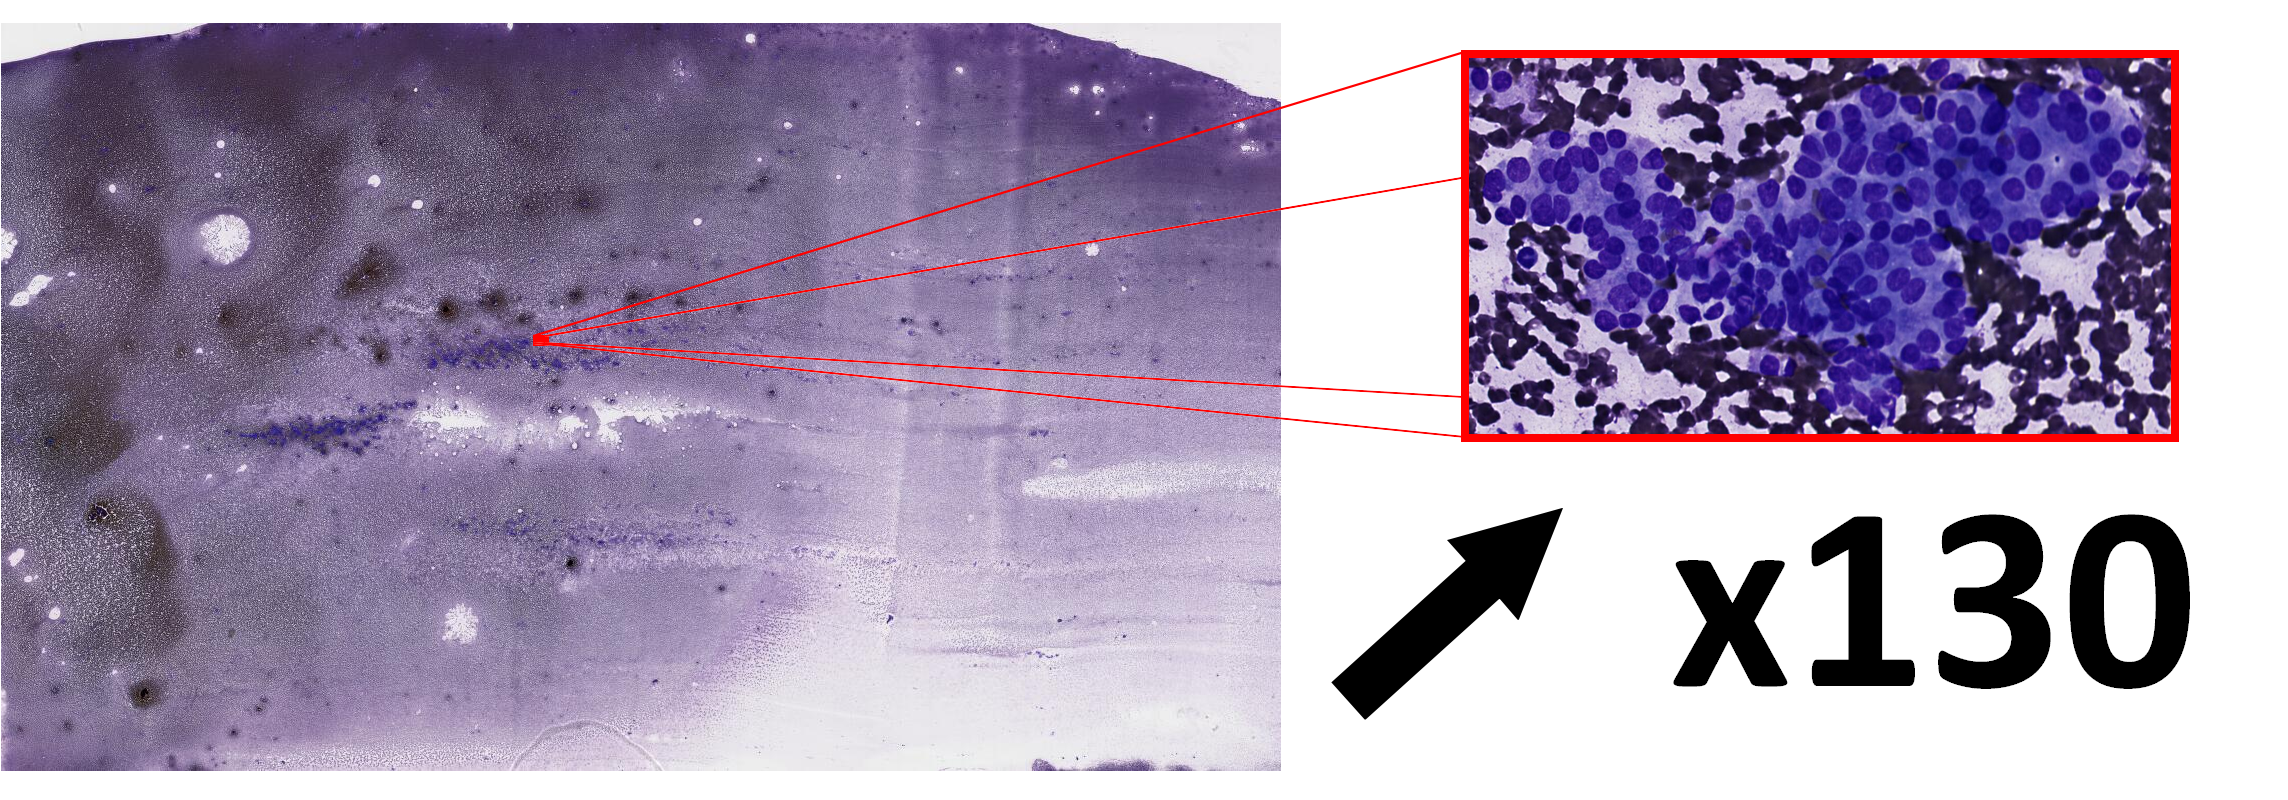
\includegraphics[scale=0.17]{images/whole-slide-dim.png}
	\caption{Microscope slide smeared with cell samples (15 gigapixels).}
	\end{figure}
	\vfill
\end{frame}


\begin{frame}{Application: thyroid nodule malignancy}
	\begin{figure}
		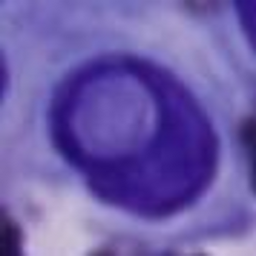
\includegraphics[scale=0.3]{images/incl1.png}
		\hspace{1cm}
		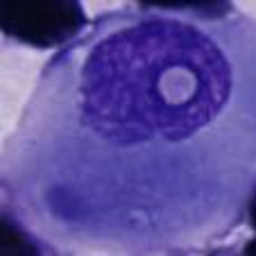
\includegraphics[scale=0.3]{images/incl2.png}
	\end{figure}
	\begin{figure}
		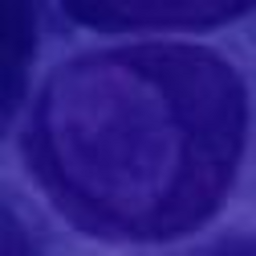
\includegraphics[scale=0.3]{images/incl3.png}
		\hspace{1cm}		
		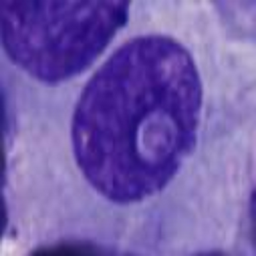
\includegraphics[scale=0.3]{images/incl4.png}
		\caption{Cells with inclusion}
	\end{figure}
\end{frame}


\begin{frame}{Application: cytology}
	\begin{figure}
		\center
		\subfigure[Proliferative]{
			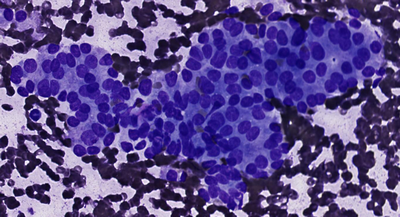
\includegraphics[scale=0.35]{images/prolif_pattern_1.png}
			\hspace{1cm}
			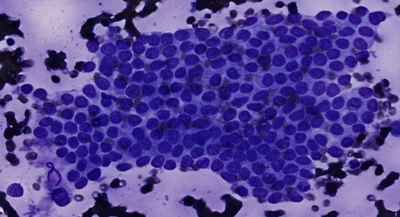
\includegraphics[scale=0.35]{images/prolif_pattern_2.png}
			\label{sfig:prolif_patterns}
		} \\
		\subfigure[Non-proliferative]{
			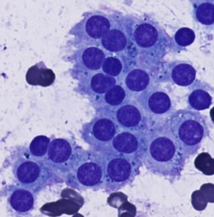
\includegraphics[scale=0.35]{images/normal_pattern_1.png}
			\hspace{1cm}
			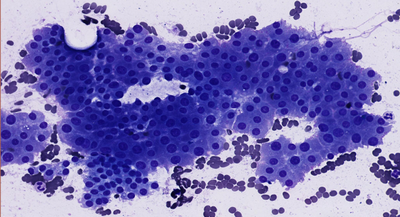
\includegraphics[scale=0.35]{images/normal_pattern_2.png}
			\label{sfig:norm_patterns}
		}
		\caption{Architectural patterns}
	\end{figure}
\end{frame}


\begin{frame}{Application: geology}
	\begin{itemize}
		\item \textbf{Aim}: assess the effects of climate variations by analysing core samples
		\item \textbf{How}: evaluate concentrations of micro-organisms present in the core samples
		\item Core samples are smeared onto microscope glass slides and \textbf{micro-organisms are manually counted by geologists}
	\end{itemize}
	\begin{figure}
		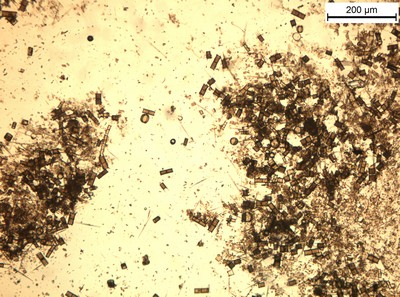
\includegraphics[scale=0.35]{images/diatomee-1.jpg}
		\hspace{1cm}
		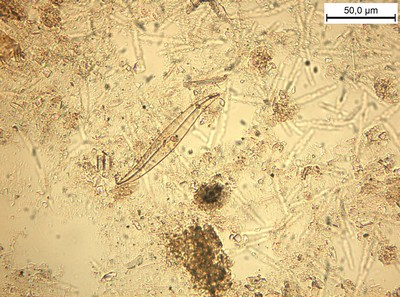
\includegraphics[scale=0.35]{images/diatomee-2.jpg}
		\caption{Example of micro-organisms (diatoms)}	
	\end{figure}
\end{frame}

\begin{frame}{Application: geology}
	\begin{figure}
		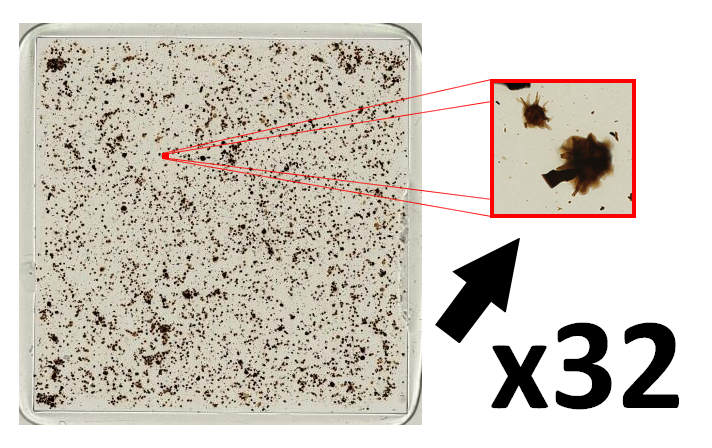
\includegraphics[scale=0.8]{images/whole-slide-geo-2.png}
		\caption{Microscope slide with smeared core samples.}
	\end{figure}
\end{frame}


\begin{frame}{Applications}
	\begin{center}
		\Large
		Both applications can be expressed as problems of \textbf{object detection and classification} !
	\end{center}	
\end{frame}

\begin{frame}{Objectives}

	\begin{enumerate}
		\item \textbf{Developing a framework} for performing object detection and classification in multi-gigapixel images
		\vspace{1cm}
		\item \textbf{Applying this framework} to the problem of thyroid malignancy diagnosis
	\end{enumerate}

\end{frame}


\begin{frame}{SLDC framework}
	\textbf{Design goals}:
	\begin{itemize}
		\item Genericity
		\item Efficiency
		\item Memory constraint (images do not fit into memory)
		\item Robustness
		\item Parallelism
		\item Ease of use and conciseness
	\end{itemize}
\end{frame}


\begin{frame}{SLDC framework: algorithms (workflow)}
	\begin{figure}
		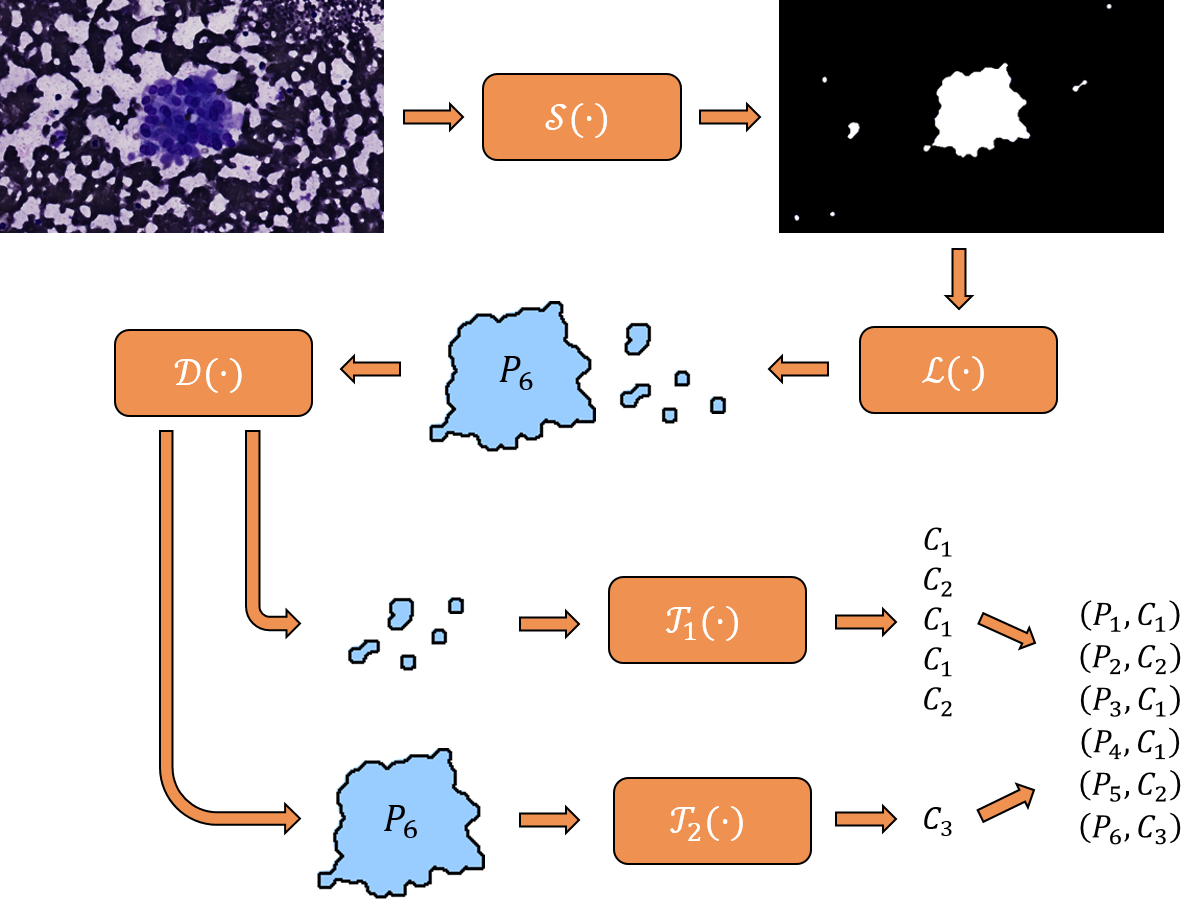
\includegraphics[scale=0.45]{images/workflow_illustration.png}
	\end{figure}
\end{frame}


\begin{frame}{SLDC framework: algorithms (chaining)}
	\begin{figure}
		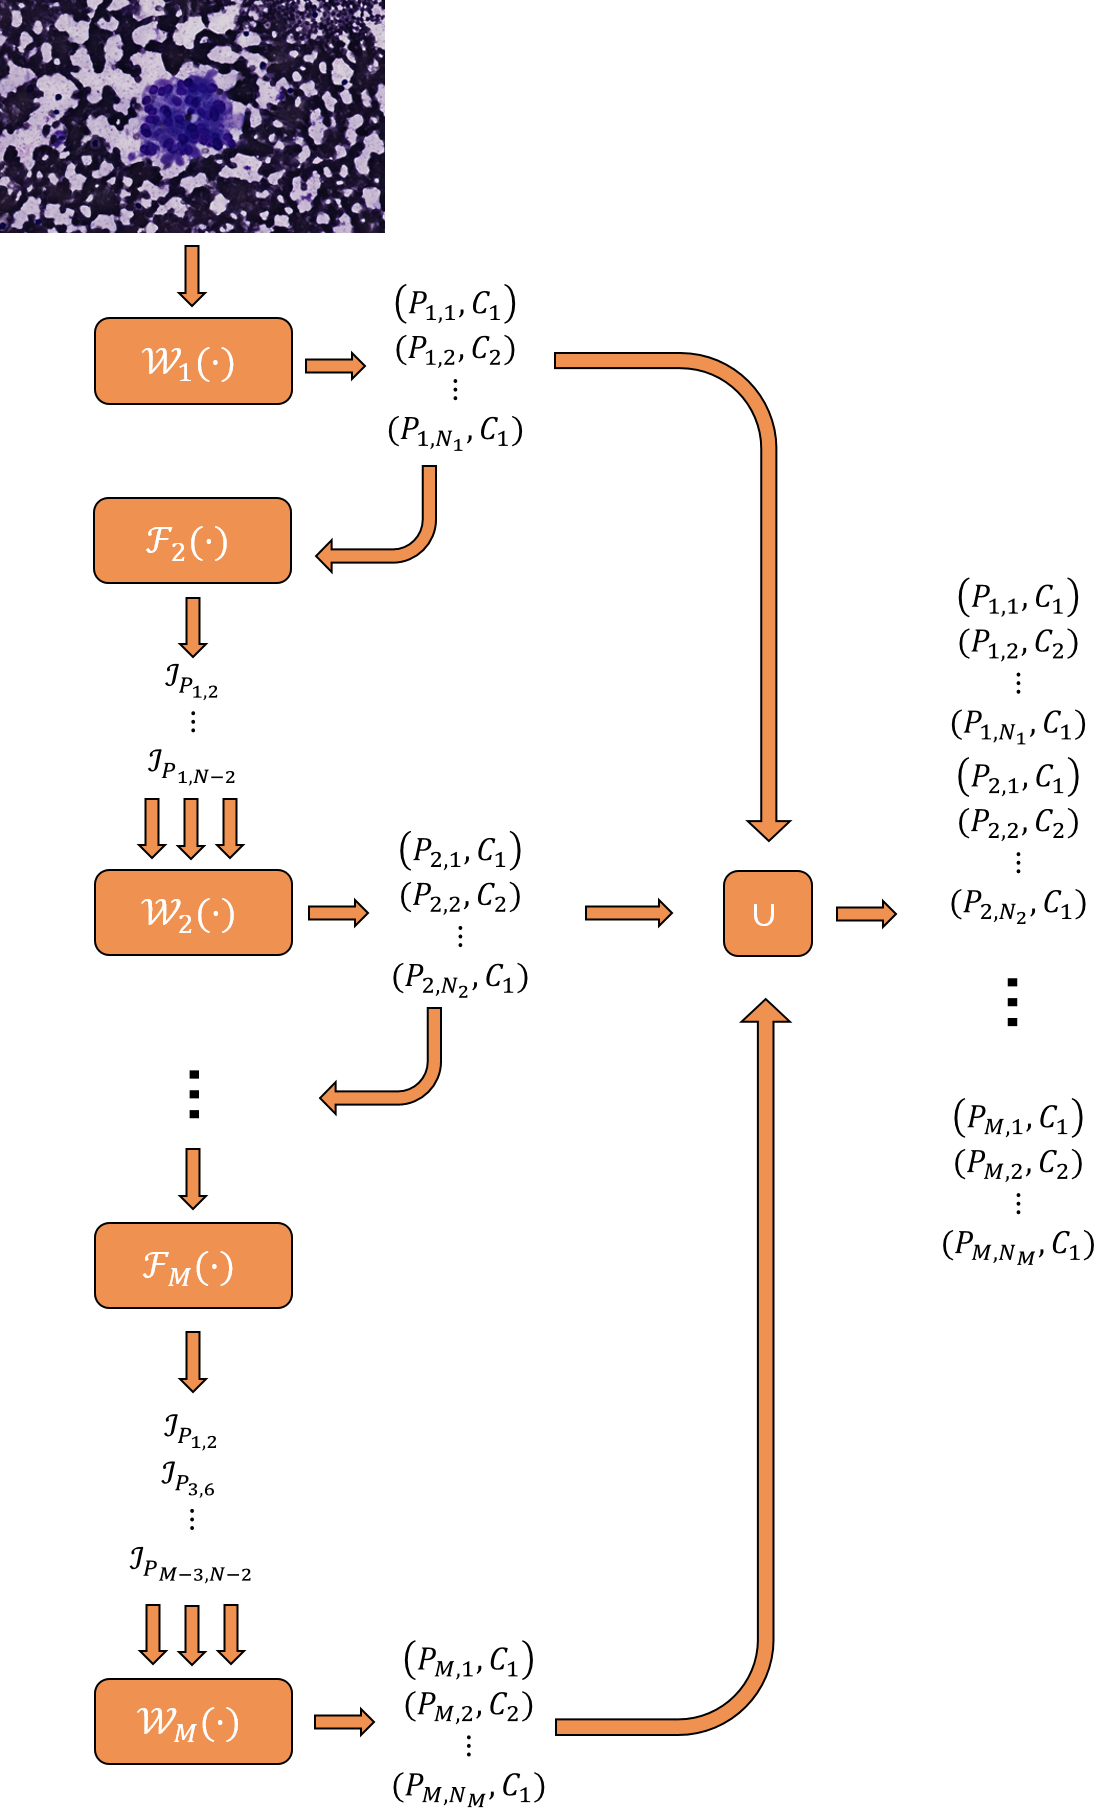
\includegraphics[scale=0.25]{images/chaining_illustration.png}
	\end{figure}
\end{frame}

\begin{frame}{SLDC framework: implementation}
	Key features:
	\begin{itemize}
		\item Memory constraint handled by \textbf{splitting images into tiles}
		\item Customizable \textbf{logging system} allowing user to keep track of execution progress
		\item \textbf{Several levels of parallelism} available 
		\item \textbf{Builder components} providing an easy way of building complex workflows
	\end{itemize}
	\vspace{0.5cm}
	About the implementation: 
	\begin{itemize}
		\item Implemented as a Python library
		\item Available on GitHub at {\small\url{https://github.com/waliens/sldc}}
		\item Unit-tested (coverage of 85 \%)
		\vspace{0.5cm}
	\end{itemize}
\end{frame}

\begin{frame}{SLDC framework: toy example}
	The aim is to detect \textbf{shape and color} of the objects in the following image:
	\vfill
	\begin{figure}
		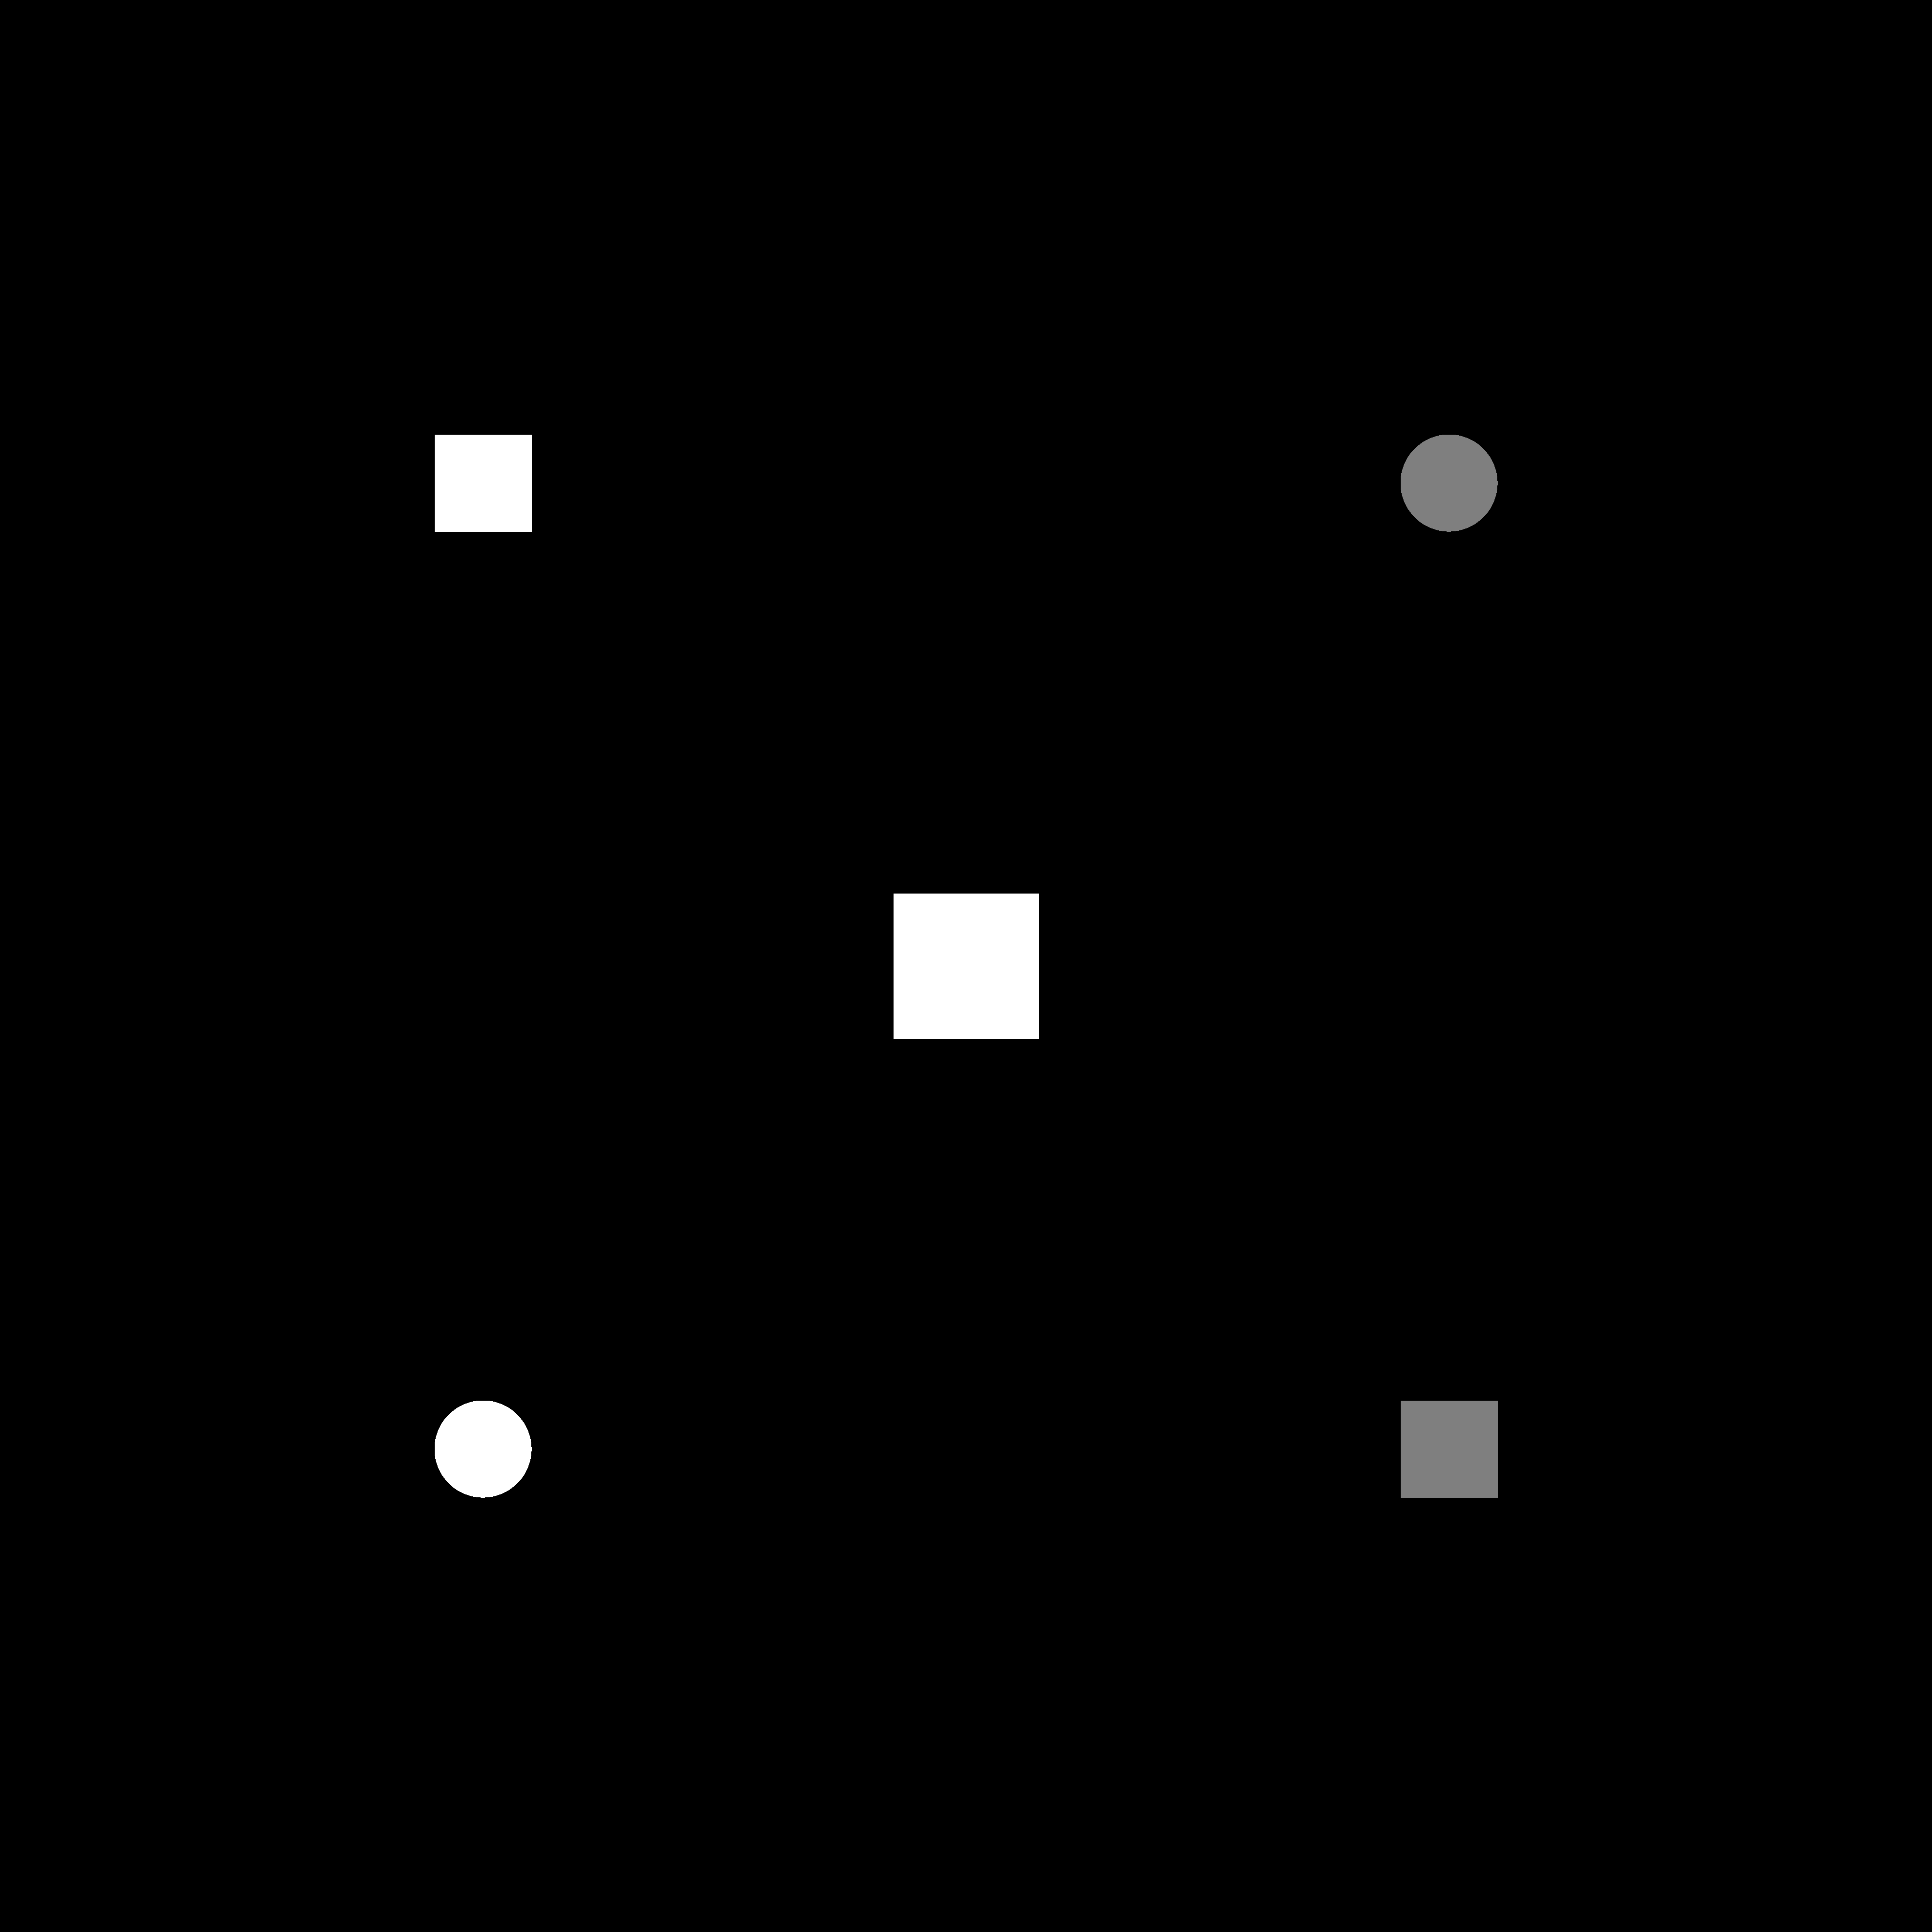
\includegraphics[scale=0.03]{images/toy_example.png}
	\end{figure}
	\vfill
\end{frame}


\begin{frame}[fragile]{SLDC framework: toy example}
\begin{minted}[fontsize=\scriptsize]{python}
# Defining a dispatching rule 
class CircleRule(DispatchingRule):
    """A rule which matches circle polygons"""
    def evaluate_batch(self, image, polygons):
        return [circularity(p) > 0.85 for p in polygons]

# Defining a segmenter
class CustomSegementer(Segmenter):
    """Every non black pixel are in an object of interest"""
    def segment(self, image):
        return (image > 0).astype(np.uint8)
        
# Defining a polygon classifier
class ColorClassifier(PolygonClassifier):
    """A classifier which returns the color class of the center 
    point of the polygon
    """
    def predict_batch(self, image, polygons):
        classes = [center_pxl_color(image, p) for p in polygons]
        probas = [1.0] * len(polygons)
        return classes, probas
\end{minted}
\end{frame}


\begin{frame}[fragile]{SLDC framework: toy example}
\begin{minted}[fontsize=\scriptsize]{python}
# Build the workflow
builder = WorkflowBuilder()
builder.set_n_jobs(4)
builder.set_segmenter(CustomSegementer())
builder.add_classifier(CircleRule(), ColorClassifier(), disp_label="circle")
builder.add_classifier(SquareRule(), ColorClassifier(), disp_label="square")
workflow = builder.get()

# Process an image
results = workflow.process(image)

# Go through the detected objects
for polygon, dispatch, label, proba in results:
  print "Detected polygon {}".format(polygon)
  print "Dispatched by '{}'".format(dispatch)
  print "Predicted class {}".format(label)
  print "Probability {}".format(proba)
  print ""
\end{minted}
\end{frame}


\begin{frame}[fragile]{SLDC framework: toy example}
\begin{minted}[fontsize=\scriptsize]{text}
Detected polygon POLYGON ((...))
Dispatched by 'square'
Predicted class 1
Probability 1.0

Detected polygon POLYGON ((...))
Dispatched by 'circle'
Predicted class 0
Probability 1.0

Detected polygon POLYGON ((...))
Dispatched by 'square'
Predicted class 1
Probability 1.0

Detected polygon POLYGON ((...))
Dispatched by 'circle'
Predicted class 1
Probability 1.0

Detected polygon POLYGON ((...))
Dispatched by 'square'
Predicted class 0
Probability 1.0
\end{minted}
\end{frame}


\begin{frame}{SLDC at work}
	\begin{itemize}
		\item \textbf{Reminder}: the aim is to detect cells with inclusion and proliferative architectural patterns in digitized slides smeared with cell samples
		\item The solution is based on a workflow developed in an earlier master thesis
		\item Some components of this workflow were reused as-is: 
		\begin{itemize}
			\item Slide segmentation
			\item Pattern segmentation
		\end{itemize}
		\item Some components were replaced or updated: 
		\begin{itemize}
			\item Dispatching updated
			\item Classification models
		\end{itemize}
	\end{itemize}
\end{frame}


\begin{frame}{SLDC at work: slide processing}
	\begin{figure}
		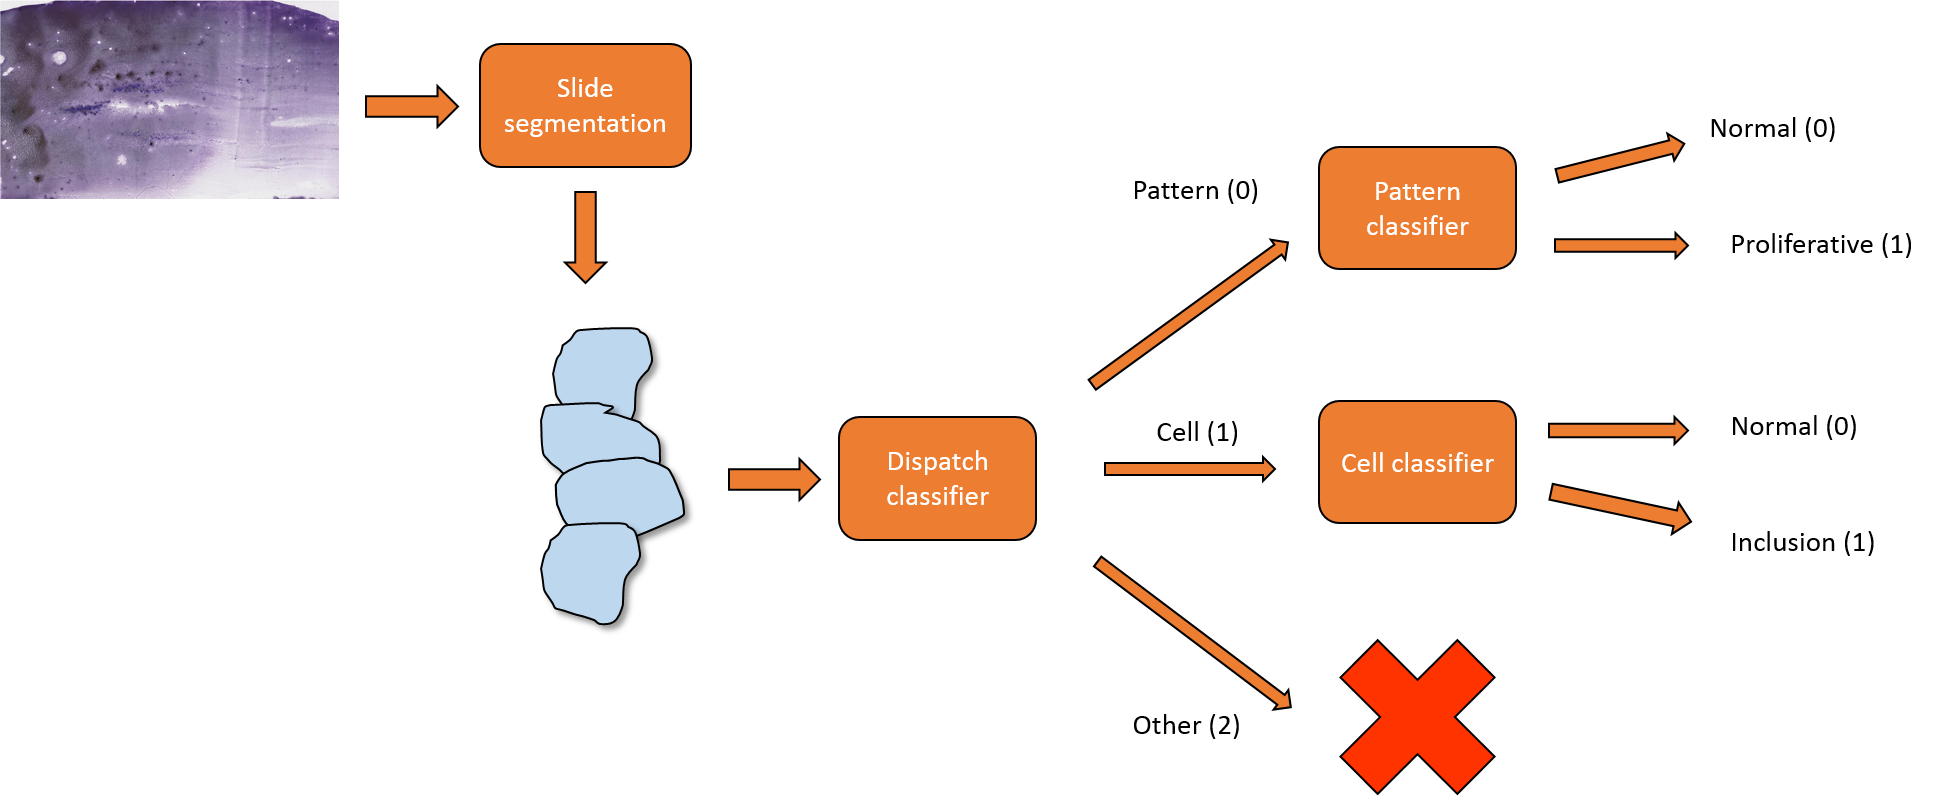
\includegraphics[scale=0.35]{images/thyroid_workflow_1.png}
	\end{figure}
\end{frame}


\begin{frame}{SLDC at work: pattern processing}
	\begin{figure}
		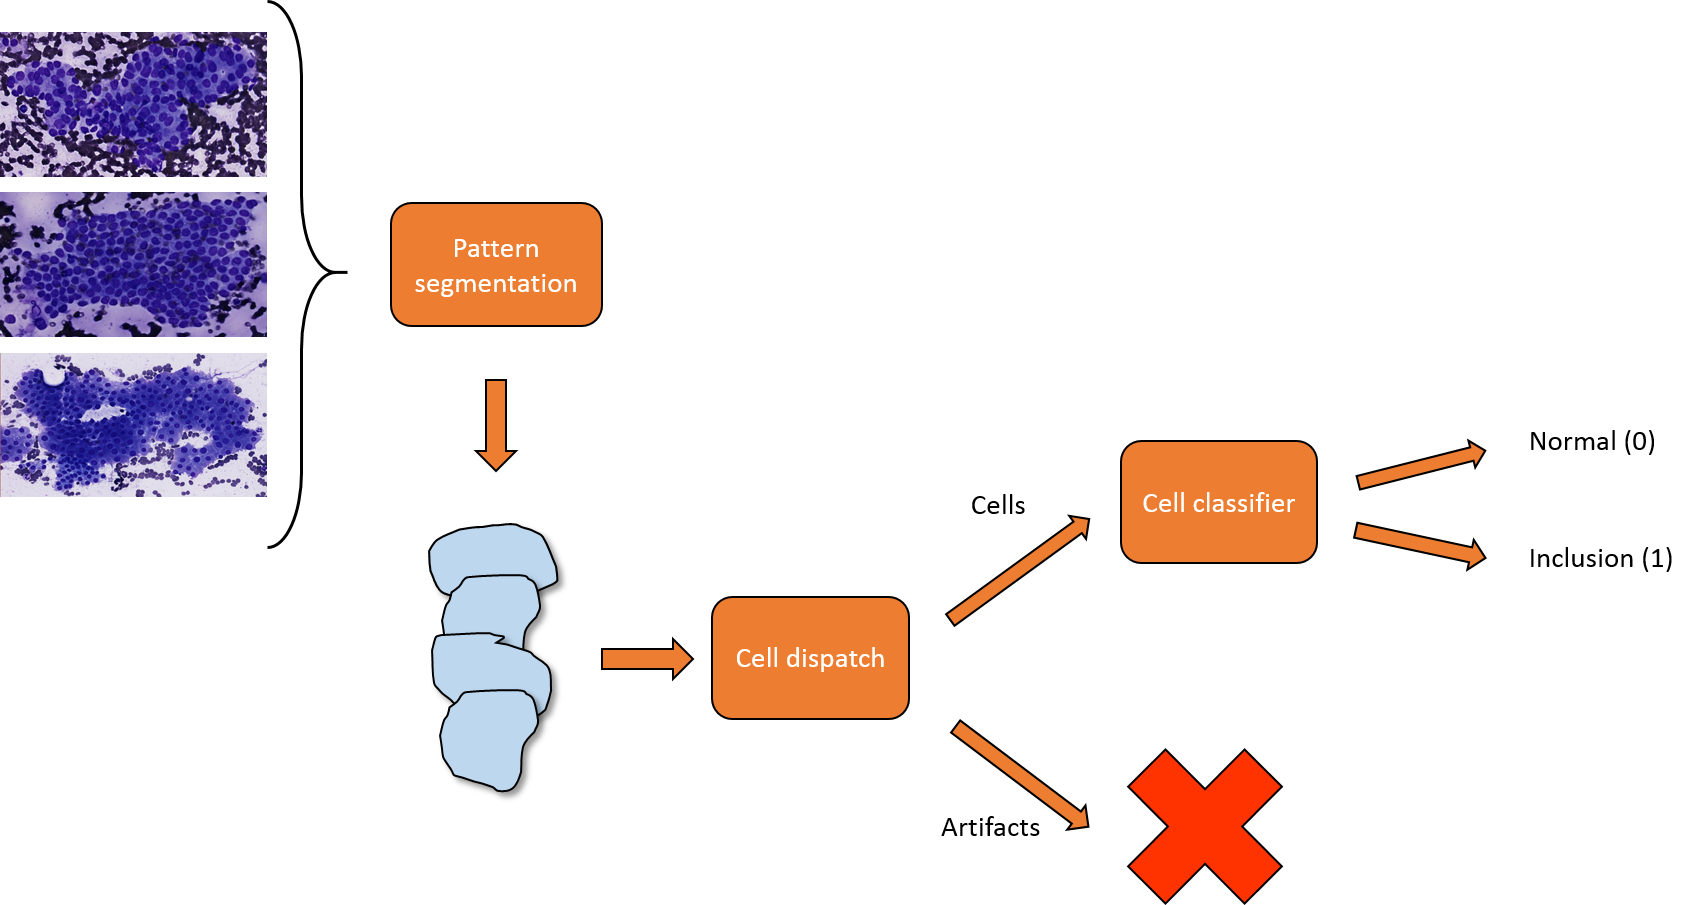
\includegraphics[scale=0.4]{images/thyroid_workflow_2.png}
	\end{figure}
\end{frame}


\begin{frame}{SLDC at work: qualitative results}
	\begin{itemize}
		\item \textbf{Slide segmentation} sometimes fails at detecting some objects but works relatively well in general
	\end{itemize}
	
	\begin{figure}
		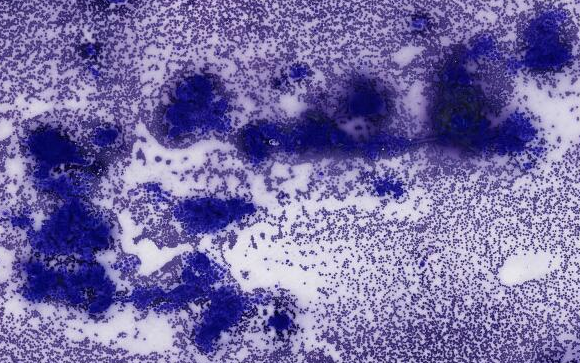
\includegraphics[scale=0.25]{images/success_pattern_1_nopat.png}
		\hspace{0.25cm}
		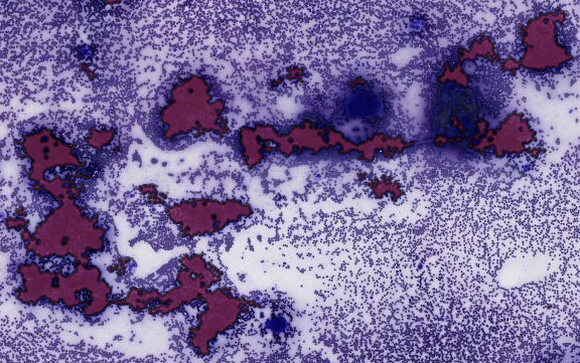
\includegraphics[scale=0.25]{images/success_pattern_1_pat.png} \\
		\vspace{0.1cm}
		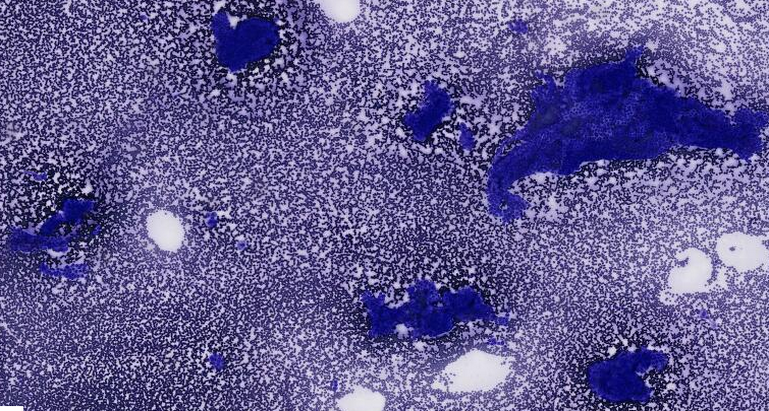
\includegraphics[scale=0.25]{images/success_pattern_2_nopat.png}
		\hspace{0.25cm}
		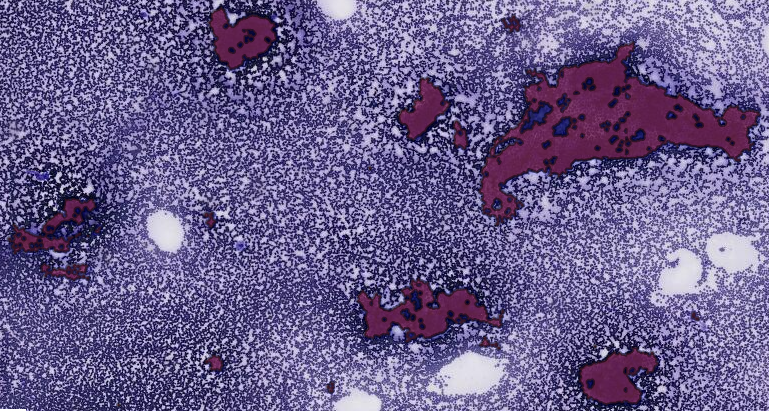
\includegraphics[scale=0.25]{images/success_pattern_2_pat.png}
	\end{figure}
\end{frame}


\begin{frame}{SLDC at work: qualitative results}
	\begin{itemize}
		\item \textbf{Pattern segmentation} works well if patterns are "\textit{clean}" on some images. Otherwise, it usually fails at detecting cells (especially cells with inclusion).
	\end{itemize}
	
	\begin{figure}
		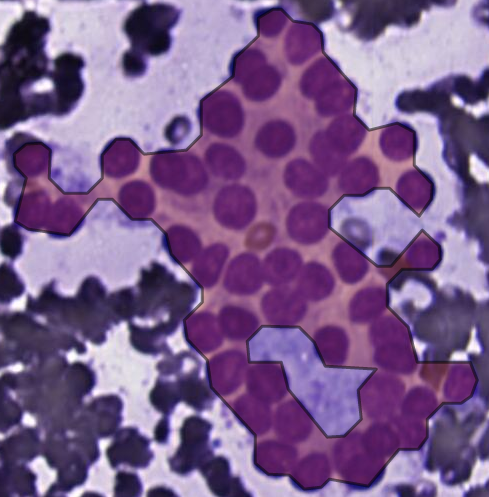
\includegraphics[scale=0.25]{images/success_reseg_2_pat.png}
		\hspace{0.25cm}
		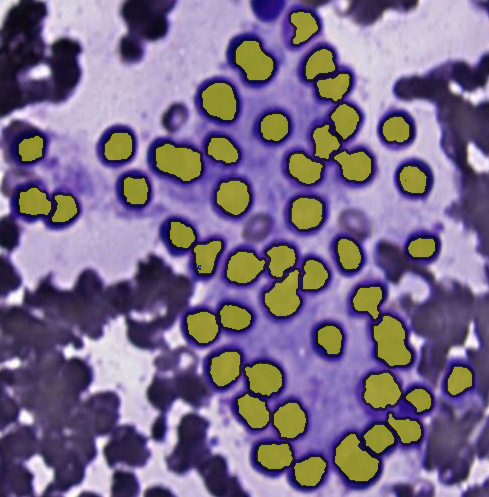
\includegraphics[scale=0.25]{images/success_reseg_2_nopat.png} \\
		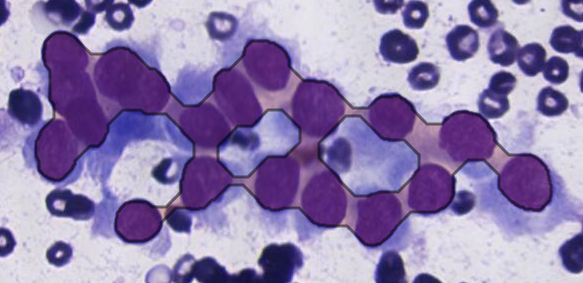
\includegraphics[scale=0.25]{images/failure_reseg_noreason_1_pat.png}
		\hspace{0.25cm}
		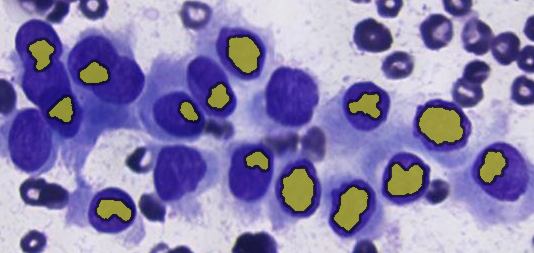
\includegraphics[scale=0.25]{images/failure_reseg_noreason_1_nopat.png}
	\end{figure}
\end{frame}


\begin{frame}{SLDC at work: qualitative results}
	\begin{itemize}
		\item The \textbf{dispatching classifier} works well as it misclassifies few objects
		\item The \textbf{pattern} and \textbf{cell classifiers} generate too many false positives and require much work
	\end{itemize}
\end{frame}

\begin{frame}{Conclusions}
	\begin{itemize}
		\item Results are promising in term of execution times: effective \textbf{processing time} of a 8 gigapixels image is approximately \textbf{8 minutes}.
		\item The \textbf{workflow developed for the thyroid problem} still fails at detecting some objects of interest and produces false positives so it \textbf{still requires some improvements}.
		\item The \textbf{framework is production-ready} and can be found on GitHub
	\end{itemize}
\end{frame}

\begin{frame}{Future works}

	\begin{block}{SLDC framework}
		\begin{itemize}
			\item Implement another structure for dispatching
			\item Improve memory consumption of the workflow
			\item Fix location algorithm
		\end{itemize}
	\end{block}
		
	\begin{block}{Thyroid workflow}
		\begin{itemize}
			\item Improve or replace both segmentation procedures
			\item Improve the classification models, especially the \textit{inclusion vs. normal}
		\end{itemize}
	\end{block}
		
\end{frame}
\begin{frame}
	\vfill
	\begin{center}
		Thank you for your attention ! \\
		Any question ?
	\end{center}
	\vfill
\end{frame}

\end{document}